\chapter{General Purpose computing with Graphics Processing Units and the GPUE codebase}
\label{ch:gpu}

The Graphics Processing Unit (GPU) is a computing card that connects to the motherboard through a Peripheral Component Interconnect Express (PCIE) slot.
As the name implies, the GPU is designed to rapidly manipulate data to create images or graphics that are sent to a display device, such as a monitor.
Because individual pixels in images are independent of each other and modern computers require updating all pixels on the display device quickly, the GPU has been developed as a massively parallel computing device, capable of efficiently performing simple tasks (such as pixel generation or manipulation) rapidly by distributing the computation among many computing cores.
This design methodology starkly contrasts the few, powerful cores on the Central Processing Unit (CPU), which is the default computing device on modern computing systems.
Due to this difference in hardware design, there are also several optimizations to consider when programming for massively parallel GPU devices, and several of these techniques will be covered in this chapter.

As GPU technology grew, other areas of computational science became increasingly hungry for computing power, specifically in the area of scientific computing on High-Performance Computing (HPC) systems.
Historically, HPC systems were often developed as large, distributed networks of computing nodes intended for CPU-based computation.
As such, these systems facilitated the development of highly parallel and distributed numerical methods to perform scientific computation.

With new, parallel algorithms being developed for HPC systems and GPU technology advancing rapidly to perform more computation in parallel to satiate the consumer demands for high-quality videos and graphics for video games and other media, it became possible to use the GPU as a scientific computing device as well with a new technique called General Purpose computing on Graphics Processing Units (GPGPU).
Modern HPC design often incorporates the GPU into each computing node, thereby increasing the throughput of the system, overall.
The fastest known supercomputer today (Summit, ORNL~\cite{kahle2019}), is entirely composed of GPU nodes with NVIDIA Tesla V100 cards (32 GB of available RAM), connected with NVlink and IBM's power architecture.
In addition to the utility of GPGPU for scientific computing, GPU technology has also been rapidly developed for AI and related fields.

In this chapter, I will discuss the design methodology for the hardware and software related to GPGPU before proceeding to the development of GPUE, the GPU-based Gross-Pitaevskii Equation solver, which will be used for the remainder of this work.
To start, I will first look into different types of parallelism and how these affect different hardware and software practices.

\section{Types of parallelism}

Older CPU architecture with a single core was designed as SISD (Single Instruction, Single Data) according to Flynn's taxonomy~\cite{gurd1988}. 
This simply means that no parallelism exists in the instructions or data.
Even now, most code is na\"ively written as if it is to be executed on SISD architecture, even though it is rare to find such a system in modern environments.
For capable devices, there are two separate methods to parallelize computation: \textit{task parallelism} and \textit{data parallelism}.

Task parallelism allows programmers to split their computation along separate, non-interacting \textit{tasks} or instructions, where each core performs its designated computation before moving on.
On the other hand, data parallelism allows programmers to perform the same, repetitive task along a large data set by distributing worker threads across the data.
Task parallelism is often better for dealing with a large number of specific actors, while data parallelism is often better for dealing with a large number of similar tasks on the same data, such as operations on a large matrix.
If a computing architecture allows for multiple instructions, but only a single data stream, it is considered to be MISD (Multiple Instruction, Single Data) by Flynn's taxonomy; meanwhile, if the architecture allows for multiple data streams with only a single instruction, it is considered to be SIMD (Single Instruction, Multiple Data).
Most modern HPC systems are designed to be MIMD (Multiple Instruction, Multiple Data), and both task and data parallelism is exploited by developers; however, for GPU computation, data parallelism is used more frequently.

In the realm of data parallelism, there is an extreme case where the data is \textit{embarrassingly parallel}.
Here, there could be a large matrix of data to manipulate, but no single element depends on any other.
This means that when distributing computation along this matrix, we can simply assign tasks to each core without considering interactions with the rest of the data set.
In this way, it is embarrassingly easy to parallelize, and hence the term \textit{embarrassingly parallel}.
As a note, element-wise matrix multiplications are embarrassingly parallel operations; however, FFTs are not~\cite{czechowski2012}.
As such, the SSFM is not overall embarrassingly parallel; however, because the FFTs are handled by the CuFFT library, programmers do not often need to consider task parallelism at all when developing SSFM code.
Even so, understanding all the features of GPUE and its future directions requires a strong understanding of GPGPU, and this will be discussed in the following section.

\section{General purpose computing with graphics processing units}

GPGPU programming is a relatively new development to the computing world and is generally much faster than CPU-based computation for tasks that can be easily parallelized in a SIMD-like fashion.
Though benchmarks vary greatly depending programming languages, code quality, and intent of the software being benchmarked, our GPUE codebase is often 5 to 10 times faster than well-optimized CPU C/C++ code and 100-200 times faster than Matlab code that is simulating the same system~\cite{wittek2016}.
This is shown in Figure~\ref{fig:bench}, where a comparison between GPUE, GPElab~\cite{antoine2014}, and Trotter-Suzuki~\cite{wittek2013} are shown for two-dimensional GPE simulations for $256 \times 256$ points for 20,000 steps in real and imaginary time using an NVIDIA Tesla C2050 and Intel i7-4790 at 3.60GHz.
These benchmarks are consistent with other GPGPU programs~\cite{garland2008, lee2010, nickolls2010}.

\begin{figure}
\center 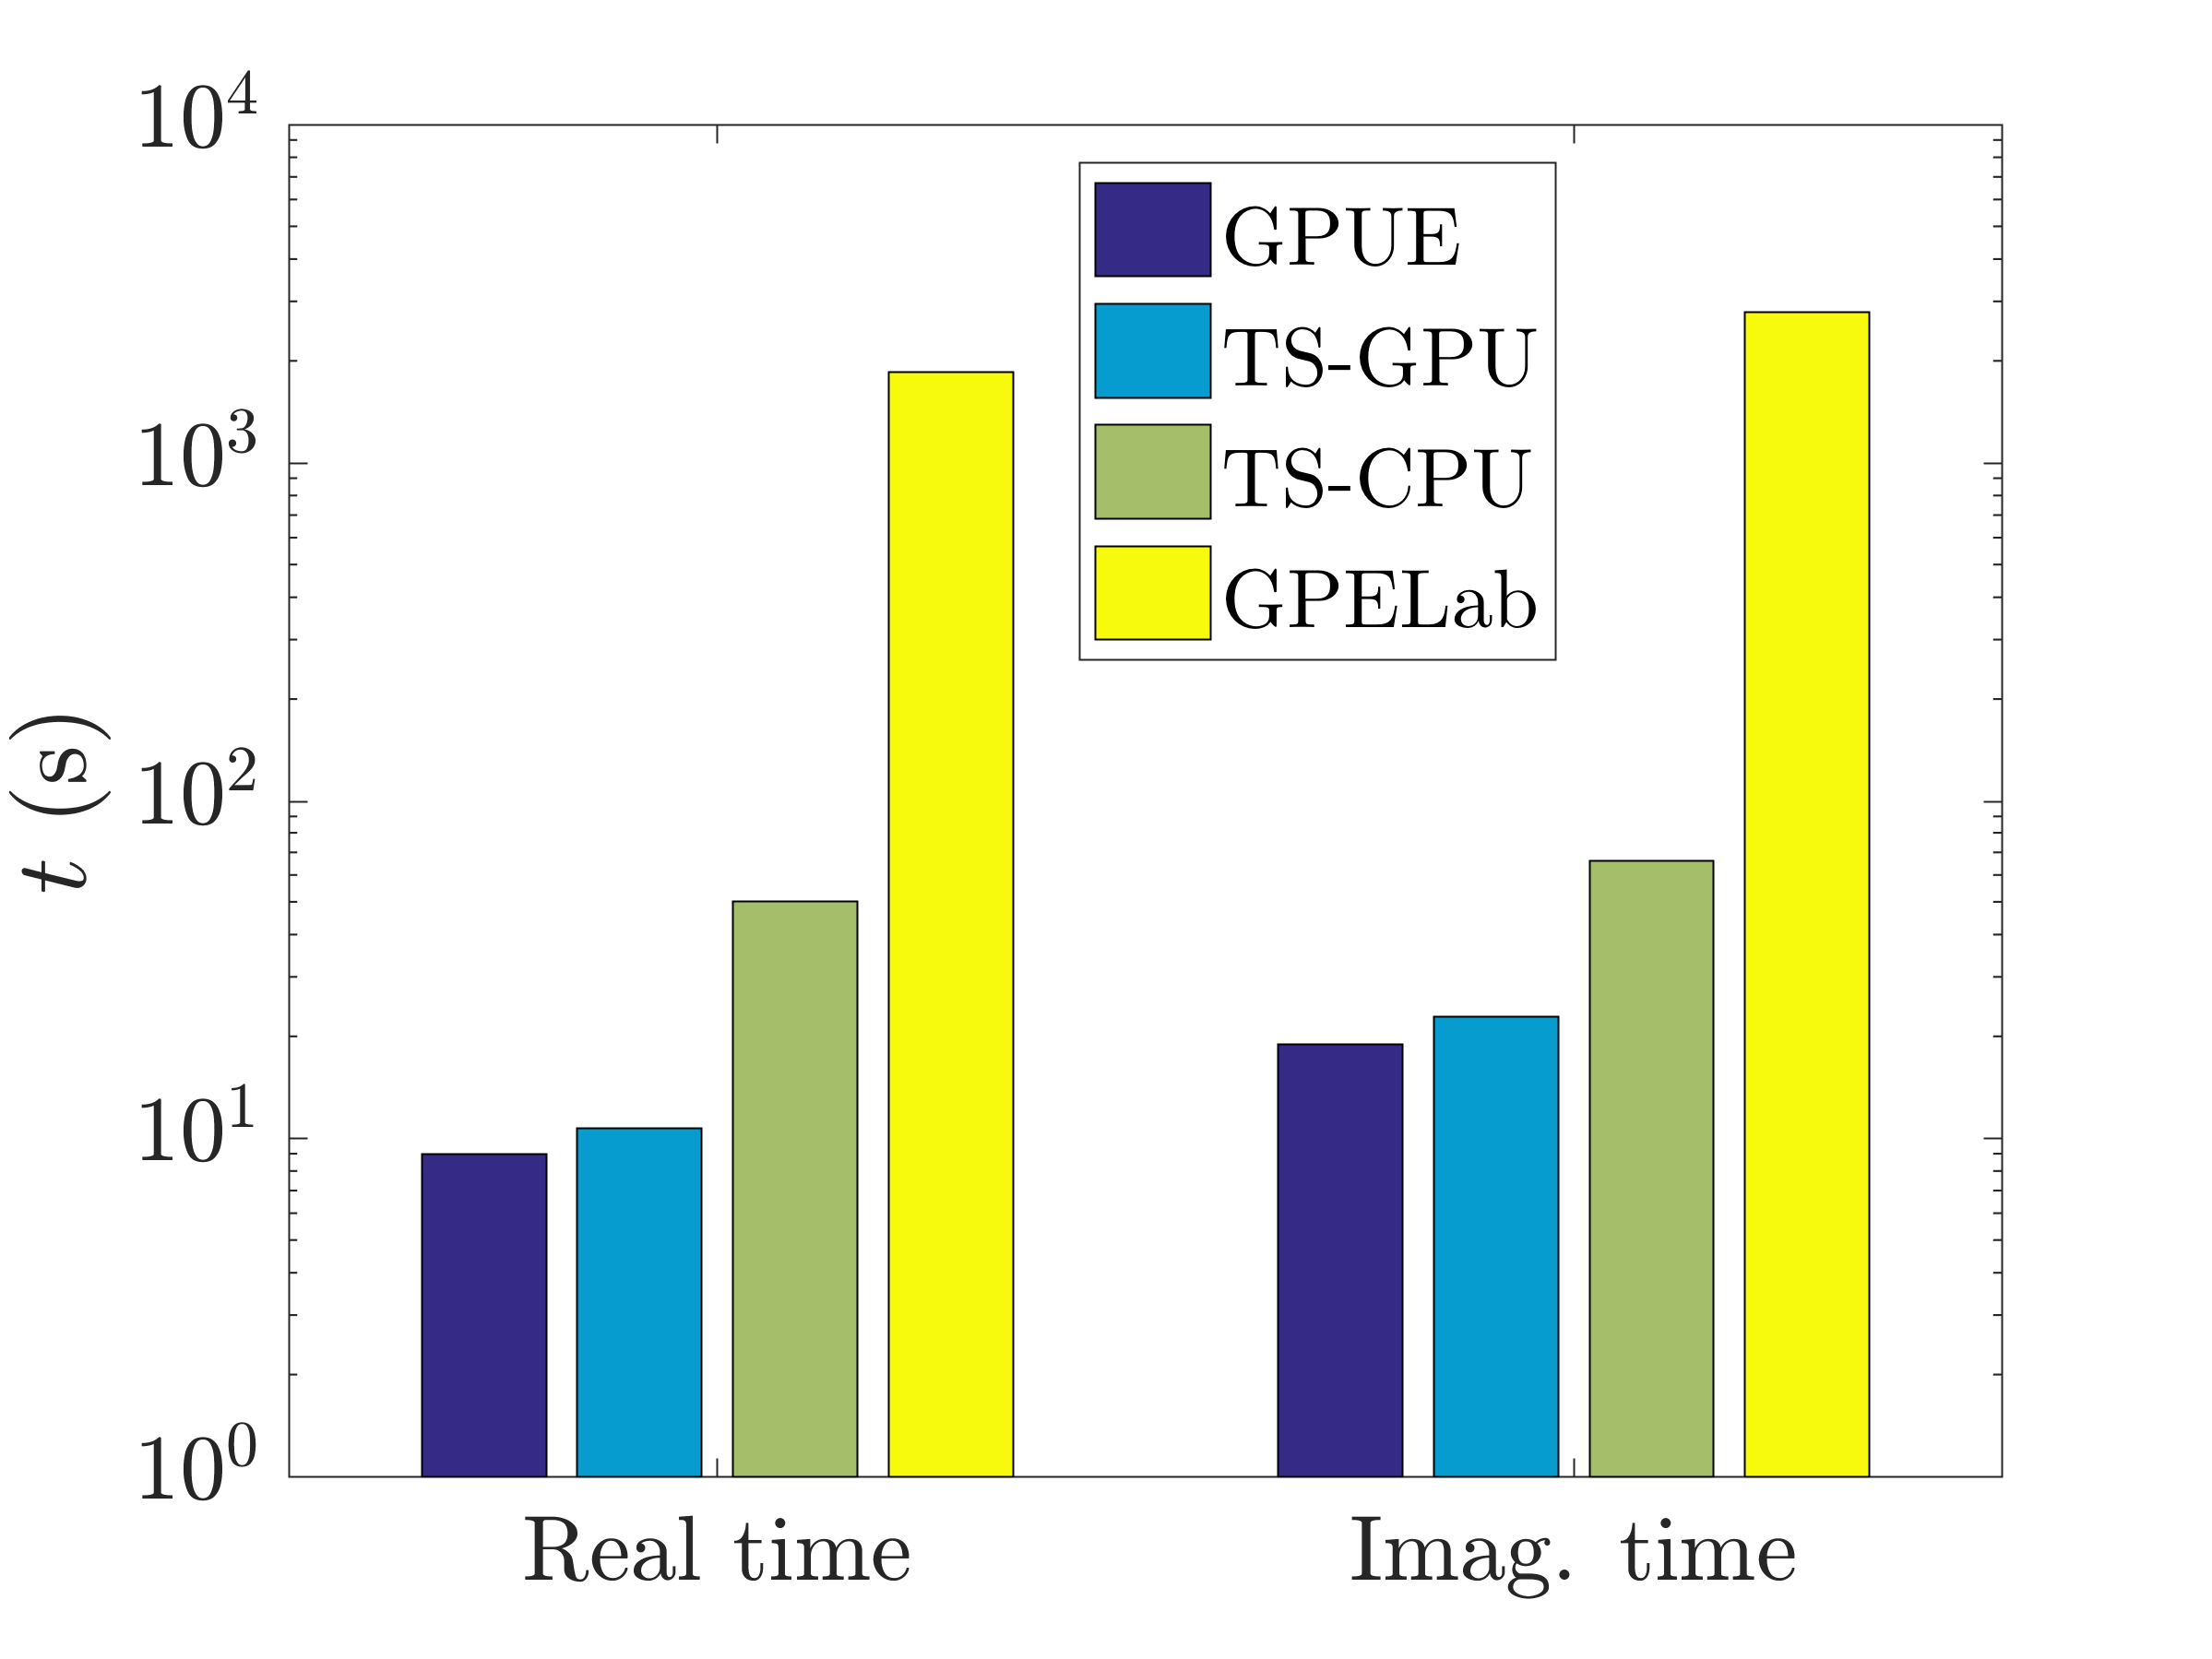
\includegraphics[width=0.5\textwidth]{data/gpu/GPUEvsTS.png}
\caption{Comparison between GPUE (CUDA), Trotter-Suzuki on both GPU (CUDA) and CPU (C++), and GPElab (Matlab).
Here, it is shown that GPUE is marginally faster than Trotter-Suzuki, but both GPU implementations are faster than the CPU-based variants.
Both software packages are much faster than GPElab~\cite{wittek2016}.
These benchmarks show two-dimensional GPE simulations for $256 \times 256$ points for 20,000 steps in real and imaginary time using an NVIDIA Tesla C2050 and Intel i7-4790 at 3.60GHz.}
\label{fig:bench}
\end{figure}

As it is possible to massively increase the performance of certain programs by using GPU hardware, it is important to discuss the differences between GPGPU and CPU-based computation, along with important optimizations for GPU computing that will be used throughout this work.
For the remainder of this work, I will use the term \textit{host} interchangeably with CPU and \textit{device} with GPU.

\subsection{Limitations of GPU computing}

GPGPU and massively parallel computation are best suited for embarrassingly parallel systems and there are several problems that are poorly suited to parallelization.
For example, any task that is inherently iterative (such as summation) or recursive (such as tree traversal) is not suited for parallel computation.
Even so, there are methods to re-frame these problems such that they are better optimized for massively parallel devices, and these will be covered when relevant to the development of GPUE.

In addition to these algorithmic limitations, GPU cards have several notable drawbacks in terms of available memory on individual cards, which is often much less than the amount available on the host.
As such, when simulating a large system on the GPU, one often limits the resolution to what can fit onto GPU memory.
In addition the data transfer between GPUs and between the GPU and CPU through the PCIE bus is a slow process.
Until recently, these limited the size of the simulated wavefunction with GPUE to roughly $512^3$ on a single Tesla K80 card.
Higher resolution simulations could be performed with more recent cards (such as the Tesla V100) or by using multiple cards; however, because it takes time to transfer data between GPUs, it is preferred to use a single card where possible.
At this point, it is worthwhile to fully discuss GPU hardware and software ideologies, with particular focus on areas relevant to the development of GPUE.
We will discuss important methods used in the development of GPUE to overcome shortcomings in GPGPU afterward in Section~\ref{sec:GPUE}.

\subsection{GPU hardware architecture}

Even though several programming frameworks exist with the capability of running code on the GPU, most of these hide necessary optimizations from the user.
As such, I have chosen to focus exclusively on programming frameworks that expose the hardware for software developers, such as CUDA, OpenCL, and Julia-GPU.
Though the following discussion will primarily focus on CUDA, a brief discussion of OpenCL and Julia can be found in Section~\ref{sec:compare}, and example code for both languages can be found in the Appendix~\ref{app:GPU}.
For the purposes of this discussion, I will cover only the GPU memory architecture of NVIDIA GPU accelerators as these are the most common computing devices for HPC systems.

This topic is easiest to describe by dividing it into two parts: an introduction to the software interface as defined by the CUDA API, followed by a discussion of the memory and thread hierarchy of GPU devices.
Throughout these sections, I will discuss performance tips to ensure maximum GPU utilization, memory throughput, and instruction throughput.

\subsubsection{Introduction to CUDA software interface}

The CUDA parallel computing platform bares the hardware of the GPU to software developers.
This means that important elements of this programming interface will appear in subsequent sections regarding hardware limitations and performance guidelines.
Much of this discussion can be found in the \textit{CUDA C Programming Guide}~\cite{CUDAPG}, while other sources will be cited as necessary.
Full code for this discussion can be found in the Appendix~\ref{app:GPU}.

\begin{lstlisting}[float,label=lst:vecadd,caption={An example of vector addition performed in C or C++ for $a$, $b$, and $c$, all of size $n$},style=c++]
for (int i = 0; i < n; ++i){
    c[i] = a[i] + b[i];
}
\end{lstlisting}

I will show a simple example where we would like to add two vectors such that $\mathbf{a} + \mathbf{b} = \mathbf{c}$.
This can be done with a simple loop in C, shown in Listing~\ref{lst:vecadd}.
In this case, we take each element with a specified index in $\mathbf{a}$ and $\mathbf{b}$ and add them to the appropriate index $\mathbf{c}$.
In some parallel programming models (OpenACC~\cite{wienke2012}, OpenMP~\cite{chandra2001}, GPUifyLoops.jl, and many others), parallelization of this method is possible by adding a pragma to the start of the loop to specify that the operation is to be performed in parallel; however, this obscures GPU hardware for the user and does not always have the same performance guarantees~\cite{reyes2012}.
As such, CUDA takes a slightly different approach by requires software developers to write \textit{kernels}, specific to the computation at hand.
An example CUDA kernel for vector addition is shown in Listing~\ref{lst:vecaddCUDA}, which has a number of notable differences to the loop in C in Listing~\ref{lst:vecaddCUDA}.
This kernel is already remarkably different than an expected function on the CPU, and it is worth comparing Listings~\ref{lst:vecadd} and \ref{lst:vecaddCUDA} in detail for a better understanding of GPU hardware.

\begin{lstlisting}[float,label=lst:vecaddCUDA, style=c++,caption=An example of a vector addition kernel in CUDA]
__global__ void vecAdd(double *a, double *b, double *c){

    // Global Thread ID
    int id = threadIdx.x;

    c[id] = a[id] + b[id];
}
\end{lstlisting}

The first peculiarity appears in line 1 with the \texttt{\_\_global\_\_} function specifier.
This is a necessary element of all CUDA kernels that specifies where and when this kernel is capable of being called.
A \texttt{\_\_global\_\_} kernel can be called by either host (with a standard CPU function) or the device (with a GPU kernel).
A \texttt{\_\_host\_\_} function is exactly the same as a CPU function and can only be called by other CPU functions.
Finally, a \texttt{\_\_device\_\_} function can only be called by other \texttt{\_\_device\_\_} functions or \texttt{\_\_global\_\_} kernels.
As a note \texttt{\_\_global\_\_} kernels are incapable of returning vectors or other variables, and must instead mutate the variables, themselves.
This is why the \texttt{\_\_global\_\_} \texttt{vecAdd(...)} kernel does not return $c$, but instead assumes it is a pre-allocated variable.
All kernels are performed asynchronously, ans special care must be taken for iterative tasks.

Another peculiarity appears on line 6, where the addition, itself, occurs.
Though there was a necessity for a loop in Listing~\ref{lst:vecadd}, there does not seem to be one at all in Listing~\ref{lst:vecaddCUDA}.
This is because the GPU is performing this task in parallel and handling the parallelism behind the scenes on line 4 with the \texttt{int id = threadIdx.x} command.
In this line, we are identifying which element of the array we are operating on with the CUDA-specific \texttt{threadIdx.x} variable.

Here, each \textit{thread} is an individual instructional element acted on in parallel with other threads in the same \textit{block}, multiple blocks are organized into \textit{grids}.
All threads in the same block have a \textit{shared memory} resource, while all three structures have access to \textit{global memory}.
In general, it is important to use shared memory when possible, as it has a lower latency than global memory, and this will be discussed further in subsequent sections.
As a note, threads often work without feedback from other threads; moreover, it may be necessary to stop thread execution until all other threads have caught up.
This can be done with the \texttt{\_\_syncthreads()} function in CUDA.

Threads, blocks, and grids are all \texttt{dim3} variables with $x$, $y$, and $z$ attributes.
The way in which these threads and blocks are allocated are defined by the user before kernel execution.
Often times, a thread number of 256, 512, or 1024 is chosen based on register usage, and the number of blocks is decided based on the size of the input array.
If there are more elements to compute than threads in a block, one then needs to use the \texttt{blockDim.x} and \texttt{blockIdx.x} variables to access the appropriate threads for computation.
Though threads may be three-dimensional in indexing, data is often indexed as one-dimensional vectors even in a multidimensional space, as shown in Figure~\ref{fig:threadsnblocks}.
Even though threads are rarely acted on sequentially, the thread ID has important ramifications that will be discussed further with other performance tips.

\begin{figure}
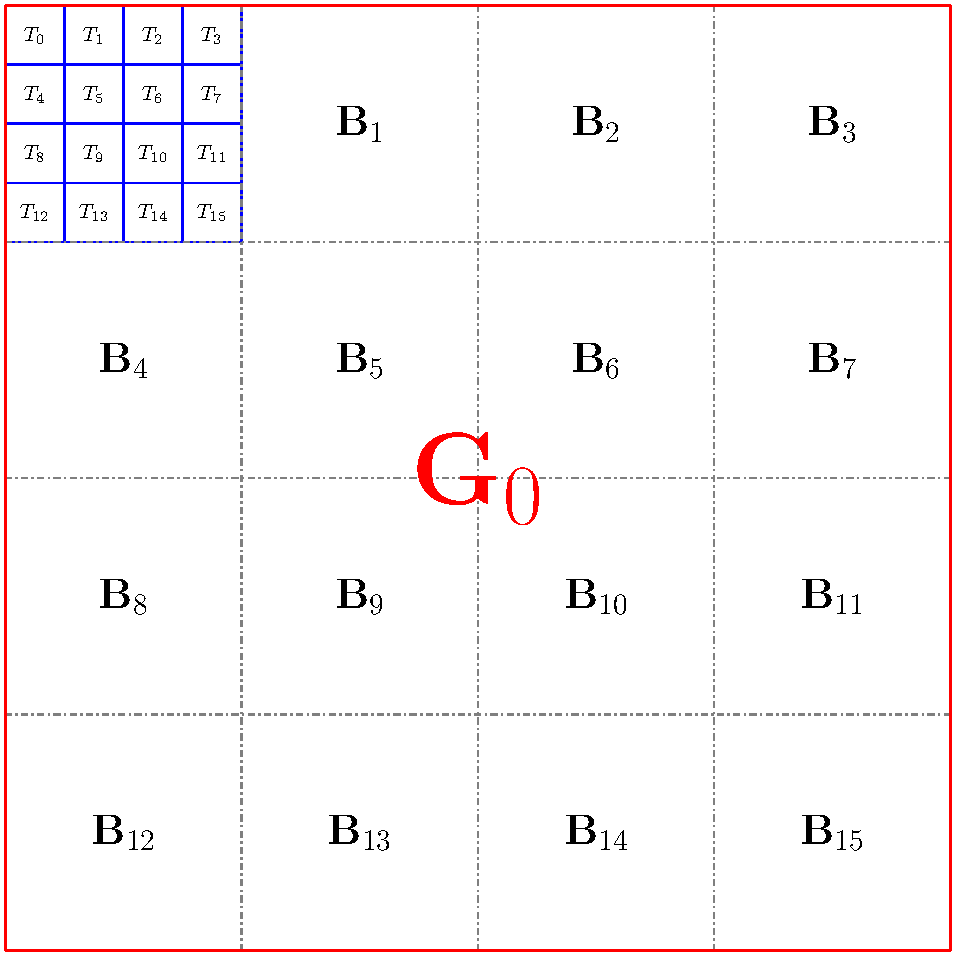
\includegraphics[width=\textwidth]{data/gpu/gputhreads.pdf}
\caption{Each grid is subdivided into multiple blocks, which is further subdivided into threads for computation. Each thread has a specified ID, which acts as a one-dimensional array, even in a two or three-dimensional system. Here, all areas outlined in red have access to global memory, and any area outlined in blue has access to shared memory.
This figure has been slightly modified from ~\cite{o2017}}
\label{fig:threadsnblocks}
\end{figure}

As another note, CUDA will execute code on unallocated memory if one does not tell it to otherwise and thus one needs to check the bounds of every computation.
As such, if one had failed to set the number of threads in the block to the number of elements in the array in Listing~\ref{lst:vecaddCUDA}, the kernel would exhibit undefined behavior.
For this reason, one needs to take into account potential out-of-bounds computation.
If one takes the above example of vector addition, assuming that the thread count is higher than can fit in one block and take into consideration potential out-of-bounds behavior, the kernel would instead look like Listing~\ref{lst:vecaddCUDA2}.

\begin{lstlisting}[float,label=lst:vecaddCUDA2, style=c++,caption={An example of a vector addition kernel in CUDA using blocks and threads, and ensuring no computation happens beyond the size of the array, $n$.}]
__global__ void vecAdd(double *a, double *b, double *c, int n){

    // Global Thread ID
    int id = blockDim.x * blockIdx.x + threadIdx.x;

    if (id < n){
        c[id] = a[id] + b[id];
    }
}
\end{lstlisting}

Finally, I need to discuss how software developers call these CUDA kernels in host code.
This requires the developer to allocate space on the device for use in the CUDA kernel via a \texttt{cudaMalloc(...)} command.
Often times, arrays on the host must also be established and transferred to the device with \texttt{cudaMemcpy(...)} functions as well.
In addition, the kernel must be configured before running with \lstinline{<<<grid, threads,...>>>}.
When everything is considered, the host code might look like what is shown in Listing~\ref{lst:vecaddhost}

\begin{lstlisting}[float,label=lst:vecaddhost, style=c++,caption={An example of host code to run Listing~\ref{lst:vecaddCUDA2}.}]
int main(){

    int n = 1024;

    // Initializing host vectors
    double *a, *b, *c;
    a = (double*)malloc(sizeof(double)*n);
    b = (double*)malloc(sizeof(double)*n);
    c = (double*)malloc(sizeof(double)*n);

    // Initializing all device vectors
    double *d_a, *d_b, *d_c;

    cudaMalloc(&d_a, sizeof(double)*n);
    cudaMalloc(&d_b, sizeof(double)*n);
    cudaMalloc(&d_c, sizeof(double)*n);

    // Initializing a and b
    for (size_t i = 0; i < n; ++i){
        a[i] = i;
        b[i] = i;
        c[i] = 0;
    }

    cudaMemcpy(d_a, a, sizeof(double)*n, cudaMemcpyHostToDevice);
    cudaMemcpy(d_b, b, sizeof(double)*n, cudaMemcpyHostToDevice);

    dim3 threads, grid;

    // threads are arbitrarily chosen
    threads = {100, 1, 1};
    grid = {(unsigned int)ceil((float)n/threads.x), 1, 1};
    vecAdd<<<grid, threads>>>(d_a, d_b, d_c, n);

    // Copying back to host
    cudaMemcpy(c, d_c, sizeof(double)*n, cudaMemcpyDeviceToHost);

    // Check to make sure everything works
    for (size_t i = 0; i < n; ++i){
        if (c[i] != a[i] + b[i]){
            std::cout << "Yo. You failed. What a loser! Ha\n";
            exit(1);
        }
    }

    std::cout << "You passed the test, congratulations!\n";

    free(a);
    free(b);
    free(c);

    cudaFree(d_a);
    cudaFree(d_b);
    cudaFree(d_c);
}
\end{lstlisting}

All said, vector addition is often known as the ``Hello World!'' of GPU programming as it is the first application that shows the parallelism of GPU devices; however, even here, a distinction between users and developers can be seen.
As more complex software is developed, it becomes more important to write software in such a way that users do not directly interface with CUDA code, and the full ramifications of this will be discussed in later in this chapter.
In addition, this discussion highlights the important distinction between host and device code, including the concept of threads and blocks, shared memory, and the ability to transfer data from the host to the device, all of which are essential to understanding particular design decisions of GPUE.
For now, I will continue this discussion by moving to GPU hardware, focusing on thread and memory hierarchy.

\subsubsection{Discussion of GPU thread and memory hierarchy}

Every time host code invokes a CUDA kernel call (as shown in Listing~\ref{lst:vecaddhost}), the data is mapped to a scalable array of multiprocessors on GPU hardware.
Multiple blocks might be distributed to the same multiprocessor, but blocks are always distributed contiguously.
Each multiprocessor is designed to execute hundreds of threads in parallel by using a unique SIMT (Single Instruction, Multiple Threads) architecture, which is similar to SIMD and can be used as such for most cases; however, there are performance benefits to optimizing instruction-level parallelism at the thread level.
Each multiprocessor distributes its parallel processes into \textit{warps}, which are units of 32 threads that execute a single common operation at a time.
Notably, the way a block is distributed into warps is always the same, so it is important to ensure that the input data is in powers of 32 to avoid wasting unnecessary computation.
Outside of this, developers can often ignore SIMT behavior as long as they do not allow threads in a warp to have separate operations.

Understanding GPU memory architecture is essential to properly using GPU hardware, and as such, it is worth discussing in-detail.
There are three forms of GPU memory that are useful for most applications of GPGPU for scientific computation: global memory, shared memory, local memory, and texture memory.
Of these memory types, local memory has the smallest scope and is only available on each individual thread.
On the other hand, global memory is shared between all grids, blocks, and threads and is considered to be the slowest memory.
As such, whenever a warp accesses global memory, it tries to perform as few accessing operations as possible, which is made easier if the warp needs to access contiguous memory blocks.
Essentially, each time a warp needs to access global memory, it tries to read a word of 1, 2, 4, 8, or 16 bytes, and
if the warp is required to access non-contiguous blocks, more accesses will be necessary and thus performance will take a relatively large hit.
This is shown in Figure~\ref{fig:coalesce}, where the size of each word is depicted as a grey box on global memory.
If each element is 1 byte, a single word is considered to be 4 bytes, and a transfer of 4 elements is required from global memory, a coalesced memory transfer corresponds to 4 consecutive elements in memory, while a strided memory transfer will not work on consecutive elements.
In this example, if the stride is 2, an additional access to global memory must be used to transfer the memory, and thus the operation will be half as optimal.
For this reason, it is important to make sure all data accesses are coalesced, which ensures that the warp will access consecutive elements as depicted in Figure~\ref{fig:threadsnblocks}.

\begin{figure}
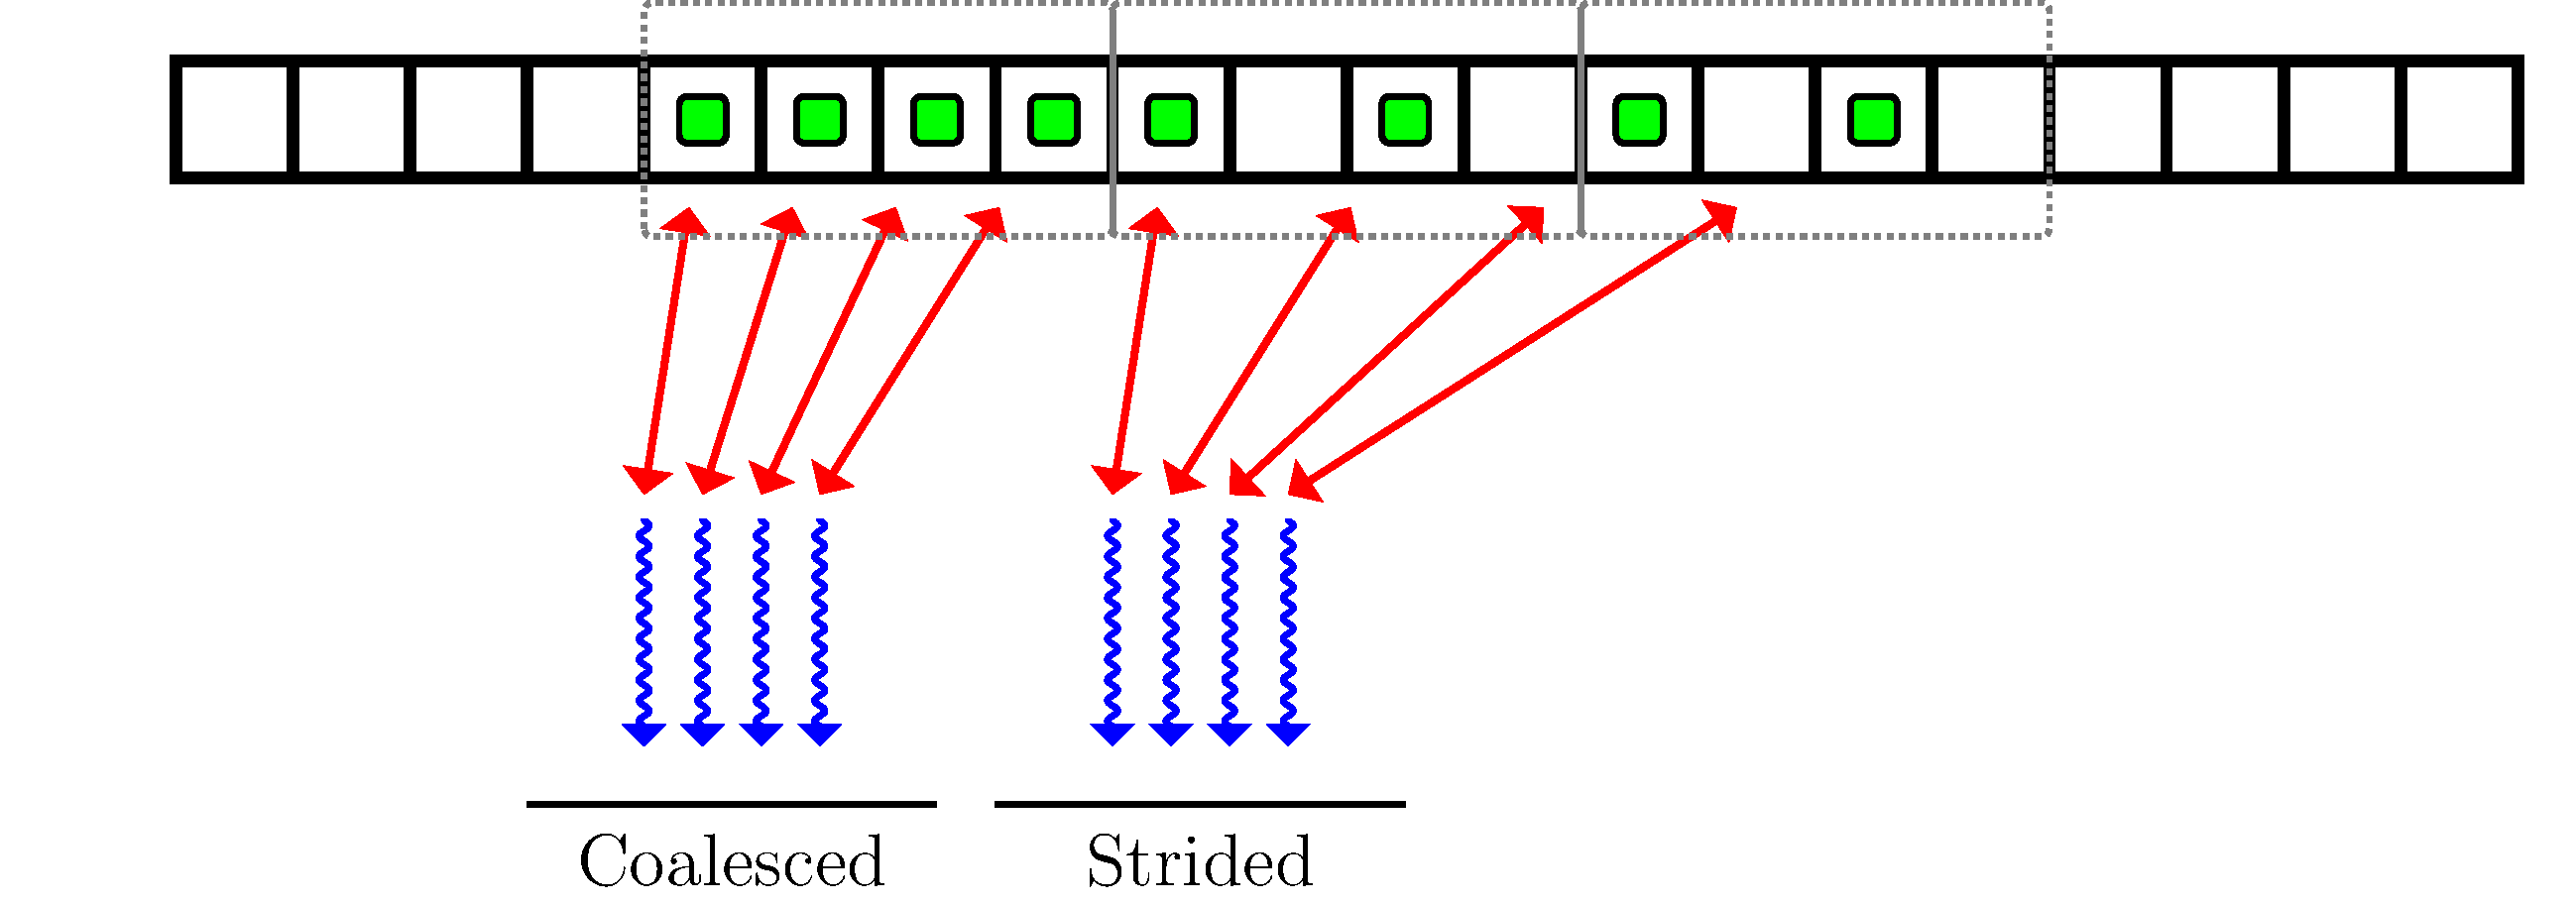
\includegraphics[width=\textwidth]{data/gpu/coalesce/check.pdf}
\caption{An example of a coalesced and strided memory transfer.
In this figure, each element is 1 byte and a single word consists of 4 bytes (grey box).
If 4 elements are required to be transferred (green boxes), a coalesced accessing patters will access 4 consecutive elements, while a strided one will not.
In this case, the strided memory access pattern requires an additional transfer and will thus be less optimal.
In this figure, worker threads are seen as blue arrows.
This figure was modified from the tikz source from~\cite{stackoverflow}.}
\label{fig:coalesce}
\end{figure}

For optimal memory throughput, shared memory is an essential tool to understand and use appropriately.
As described, shared memory is on-chip memory that is shared between all threads in a block.
The amount of shared memory available is hardware-dependent and configurable on kernel execution.
In general, it is worthwhile to transfer data with a large number of accesses to shared memory for performance.
Shared memory is split into several memory banks which can be accessed simultaneously.
If two memory accesses are required of the same bank, there will be a conflict (known as a bank conflict) and the operation can no longer be performed in parallel.
It is sometimes necessary to pad variables to prevent bank conflicts from occurring~\cite{harris2013}.

Of the four types of memory mentioned, texture memory is the least-often used and is primarily on the GPU for graphics computation and focuses on performance for two-dimensional structures.
Texture memory has a relatively long write time, but is quick to read.
It is also faster than global memory for non-coalesced access patterns and therefore can be useful for certain tasks with slowly varying operators.
In principle, this is the case for the momentum-space operator in the SSFM; however, because texture memory uses single-precision, it will not be used further in this work.

In addition to appropriate usage of memory on GPU architecture, it is also essential to minimize data transfers between the device and host and even between devices in multi-GPU setups or perform these transfers asynchronously.
The data transfer between the host and device or between devices must send data through the PCIE slot on the motherboard, which is a slow operation.
For data transfer between devices, this transfer time can be slightly alleviated on Power architecture where NVlink technology can directly transfer data from device to device~\cite{foley2017}, but the data transfer between devices will still likely be the slowest part of the computation.
In addition, CUDA-aware MPI for multi-GPU setups may greatly increase software development time~\cite{lonvcar2016, wang2013}.
As such, developers often try to keep all of their computation on a single card, if possible, and several optimization strategies are used when multiple GPU cards are needed.
These strategies will be covered on a case-by-case basis as they arise in this work.

As a final note, one optimization strategy for CUDA code that will not be discussed in-depth in this work is the maximization of instruction throughput.
The simplest optimizations here involve increasing the number of instructions performed over a specified period by trading precision for speed and minimizing thread synchronization.
Because we are performing high-precision superfluid simulations, we cannot perform a trade-off between precision and computational speed.
When optimizing the instruction throughput for GPU devices, it is important to discuss conditionals, like \texttt{if} and \texttt{switch} statements.
Here, programmers need to be careful not to accidentally cause the operation executed on threads in a warp to diverge.

\subsection{Comparison between various languages for GPGPU computation}
\label{sec:compare}

As one might expect, specialized programming languages are necessary to write code that compiles and runs on GPU architecture.
There are several known libraries to extend modern programming languages such as Matlab, Python, and C++ to GPU devices; however, we will limit this discussion to common programming methods that allow fine-grained control of GPU memory and could be used for the development of GPUE.
We will briefly discuss the advantages and disadvantages of three competing languages considered here: CUDA, OpenCL, and Julia, and as a simple example, vector addition in these languages is shown in  Appendix~\ref{app:GPU}.

\subsubsection{CUDA}
CUDA is a computing API provided by NVIDIA for interfacing with NVIDIA GPUs and is the industry standard for GPGPU programming.
CUDA is primarily limited by the NVIDIA-specific hardware it runs on, and although NVIDIA currently produces the most common GPUs for GPGPU programming, AMD GPU devices are also available and provide a similar level of computational power.
In addition, CUDA support has recently ceased for MacOS systems as NVIDIA cards are no longer bundled with current generation Mac computers, so CUDA code can only be used on Windows and Linux devices with NVIDIA cards.
GPUE was written entirely in CUDA; however, due to the aforementioned limitations, there has been some consideration to re-writing the software in OpenCL or Julia.

\subsubsection{OpenCL}

Though CUDA is the industry-standard for GPGPU programming, OpenCL (Open Compute Language) is largely competitive in terms of performance and has the benefit of being compatible with both NVIDIA and AMD GPU devices~\cite{opencl, fang2011}.
OpenCL is also completely open-source and works as additional libraries to C or C++, which allows developers to compile OpenCL code with traditional compilers like \texttt{gcc} or \texttt{clang}.
OpenCL has nearly similar structure to CUDA with slightly more verbose syntax, and thus provides all necessary functionality to develop and maintain scientific software.
It should be mentioned that OpenCL can also run on a large variety of other computing architectures, such as Field-Programmable Gate Arrays (FPGA) and is a more general-purpose computing library than CUDA.
In addition, compute kernels are compiled at run-time, meaning that users can potentially modify kernels without recompiling the code.
This could be a huge boon for developers writing software for users who may need to quickly simulate a slightly modified system.
Because OpenCL is defined as a general-purpose API with higher access to low-level functionality, it is often more cumbersome for developers than CUDA for GPGPU~\cite{komatsu2010}.
As such, it is not as widely used for scientific computing software.

In the end, although OpenCL does provide the ability to more easily construct kernels that can be compiled at runtime, the increased engineering time necessary to write software in OpenCL is often not worth the cost; however, further advances in compiler design for heterogeneous architecture has been made in the past few years \cite{besard2019}, which has provided the unique opportunity for computer scientists to write maintainable and fast code in new languages, like Julia.

\subsubsection{Julia-GPU}
Julia is a new language to scientific computing, but boasts promising results.
It claims to be as usable as Python, but as performant as C~\cite{bezanson2017}, which is beneficial for maintainability of HPC software.
In addition, Julia's runtime is comparable to CUDA C for GPGPU computation and allows for similar hardware optimizations \cite{besard2016, besard2018}, while also allowing users to edit the compiler implementations at will.
This is an important point that will be discussed in more detail in Section~\ref{sec:expr_trees}.

In addition, because Julia is much easier to write than C for new programmers, GPU-based Julia code could allow developers to provide fast, efficient code with a usable interface for scientists and engineers.
The trade off between performance and readability in programming has been described as the ``two-language'' problem, as most scientific computing solutions to this point have required using two languages: a fast language for the back-end and a readable language for the user interface.
Julia succeeds in bridging the gap between the languages, effectively solving the two-language problem and allowing scientists and engineers to write efficient code that is also compilable on the GPU.
For these reasons, we have begun porting our CUDA code to Julia, as it will lead to simpler and more maintainable code in the future.
This will be further discussed in the outlook of this work, Chapter~\ref{ch:conclusion}.
In Chapters~\ref{ch:2d} and \ref{ch:vortex_states}, I will also introduce systems that could benefit from a Julia interface.

\section{Introduction to the GPUE codebase for $n$-dimensional simulations of quantum systems on the GPU}
\label{sec:GPUE}

At this point, all the motivation and background necessary has been provided to discuss GPUE, the GPU-based Gross-Pitaevskii Equation solver.
This codebase will be used for all remaining simulations performed in this work and its development has also inspired the development of other computational libraries such as the \texttt{DistributedTranspose.jl} package, which will also be discussed in Section~\ref{sec:DT}.
Some additional information on prior development of GPUE can be found in other sources~\cite{o2017}.
The GPUE codebase was published in the \textit{Journal of Open Source Software} in 2018~\cite{schloss2018} and
was originally designed by Lee J. O'Riordan with the capability of simulating large-scale Abrikosov lattices in two-dimensional superfluid BECs~\ref{o2017, o2016, o2016topo}.
My focus with GPUE development has been to simulate three-dimensional systems and optimize the software for dynamic studies on GPU hardware.
For this section, I will first describe the FFT optimizations used in GPUE for three-dimensional simulations, followed by additional features necessary for dynamic simulations on GPU architecture.

\subsection{FFT optimization}

As mentioned in Chapter~\ref{ch:splitop} and previously in this chapter, the SSFM is primarily limited by the complexity of the FFT operations.
For a three dimensional simulation with gauge fields in the $\hat x$, $\hat y$, and $\hat z$ directions, one set of global FFTs and three sets of one-dimensional FFTs must be performed.
This is equivalent to two three-dimensional FFT operations, which become much more undesirable when scaling to multiple GPU devices~\cite{czechowski2012}.
The CuFFT API provides an option for computing FFT's on separate batches of an array in GPU memory with the \texttt{cufftPlanMany(...)} command; however, if this command is repurposed for one-dimensional FFT operations, it does not provide the necessary functionality for FFTs across the $\hat y$ or $\hat z$ dimensions.
With the CuFFT library, all FFT operations performed with this plan must follow an indexing pattern, such that 

\begin{lstlisting}
input[b*idist + x*istride]
output[b*odist + x*ostride]
\end{lstlisting}

\noindent where \texttt{b} is the batch ID, \texttt{x} is the element ID, \texttt{idist} and \texttt{odist} are the distances between batches for the input and output array, respectively, and \texttt{istride} and \texttt{ostride} are the strides between consecutive elements for computation with the input and output array, respectively.
On the other hand, if data is transferred to the GPU, it is often re-indexed as a one-dimensional array, such that

\begin{lstlisting}
array[i,j,k] = array[i + j*xDim + k*xDim*yDim]
\end{lstlisting}

\noindent where \texttt{i}, \texttt{j}, and \texttt{k} are iterable variables in the $\hat x$, $\hat y$, and $\hat z$ directions, and \texttt{xDim}, \texttt{yDim}, and \texttt{zDim} are the dimensions in $\hat x$, $\hat y$, and $\hat z$, respectively.
As such, it is not possible to use the \texttt{cufftPlanMany} functionality to perform one-dimensional FFTs in $\hat y$ and $\hat z$; however, if we increase the number of batches to \texttt{yDim*zDim}, set the distance between each stride to 1, and assume the stride between each element is \texttt{xDim*yDim}, we can recreate the functionality of the FFT in the $\hat z$ direction.
For the $\hat y$ FFT operations, we need an external loop that iterates over each $xy$ slab, performing \texttt{xDim} operations on each slab, and this greatly hampers performance.
This is depicted in Figure~\ref{fig:FFTopt} for a $2\times 2\times 2$ grid.

\begin{figure}
\center 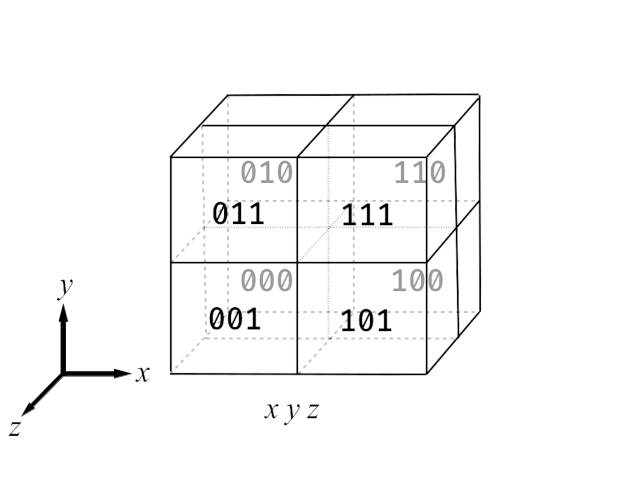
\includegraphics[width=0.5\textwidth]{data/gpu/fft/fft_fig.png}

\center 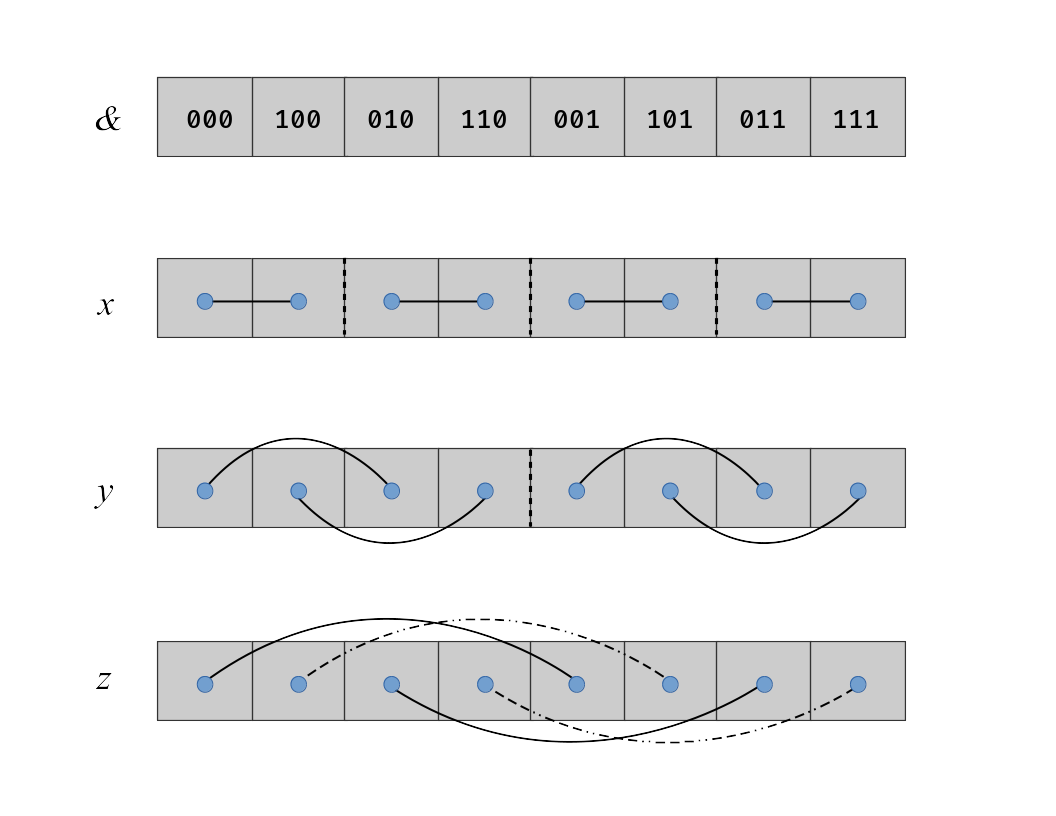
\includegraphics[width=0.9\textwidth]{data/gpu/fft/fft_fig2.png}

\caption{An example 2$^3$ data cube with indices 000$\rightarrow$111 with stride and batches shown for $x$, $y$, and $z$ FFTs.
For the $x$ FFT, the stride is 1, the batch number is 4, and the distance between each batch is 2.
For the $z$ FFT, the stride is 4, the batch number is 4, and the distance between each batch is 1.
Here, every other line is dashed for visualization.
These two transforms can be performed with the \texttt{cufftPlanMany} functionality.
For the $y$ FFT, the stride should be 2, and the number of batches should be 4; however, no matter what one specifies the distance between each batch to be, it is not possible to perform the operation.
This figure can be found in the GPUE documentation~\cite{docs}.
}
\label{fig:FFTopt}
\end{figure}

With this considered, only one-third of the necessary FFT operations are appropriately coalesced in memory for three dimensional simulations.
Because FFTs are global operations that are best performed on contiguous chunks of memory, multi-GPU simulations with the SSFM are even less optimal.
This has motivated the development of other packages to allow for memory coalescence with FFT operations, such as the distributed transpose, which will be described in Section~\ref{sec:DT}.
Even though the three-dimensional FFT operations are the biggest bottleneck in the GPUE codebase, it is not easy to avoid usage of the \texttt{cufftPlanMany(...)} operation while still using CUDA.
This is why optimizations to GPUE FFT operations will be performed exclusively in GPUE.jl.
Next, I will focus on another feature that was inhibited by the CUDA framework, but is nevertheless possible: methods to enable dynamic quantum state engineering with expression trees.

\subsection{Dynamic field input and output in GPUE with expression trees}

\label{sec:expr_trees}
As mentioned in Chapter~\ref{ch:1d}, quantum state engineering typically requires some form of time-dependent variables, along with evolution in real time.
This means that the user must be able to input a time-dependent equation to GPUE, often for $V(t)$, $g(t)$, or $\mathbf{A}(t)$.
Because GPUE is written in C/C++ and CUDA, there is no straightforward method for the user to input time-dependent fields without recompiling the source code and modifying CUDA kernels at will, which is unnecessarily cumbersome for the user.
As such, we have provided a method for users to input the fields of their choosing as strings, which will be compiled into a set of operations to perform on the GPU through expression trees, which are similar to Abstract Syntax Trees (ASTs) in compiler design~\cite{cohen1991, reyes2011}.

\begin{figure}
\center %\documentclass{article}
%\usepackage{tikz}
\usetikzlibrary{arrows}
\tikzset{
  exprnode/.style = {align=center, inner sep=0pt, text centered,
    circle, draw=black, text width=1.5em},
  varnode/.style = {exprnode, red, draw=red},
  posnode/.style = {exprnode, green!50!black, draw=green!50!black},
  oprnode/.style = {rectangle, white, draw = blue, fill=blue},
}
%\begin{document}
  $V = \frac{1}{2}m\omega^2 x^2 t$
  
  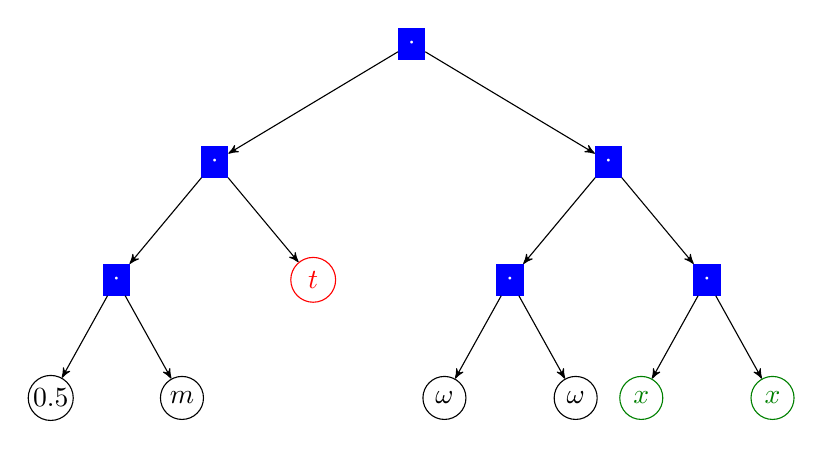
\begin{tikzpicture}[->,>=stealth',level/.style={sibling distance = 5cm/#1,
    level distance = 1.5cm}]
    \node [oprnode] {$\cdot$}
      child{ node [oprnode] {$\cdot$}
        child{ node [oprnode] {$\cdot$}
          child{ node [exprnode] {$0.5$}}
          child{ node [exprnode] {$m$}}
        }
        child{ node [varnode] {$t$}}
      }
      child{ node [oprnode] {$\cdot$}
        child{ node [oprnode] {$\cdot$}
          child{ node [exprnode] {$\omega$}}
          child{ node [exprnode] {$\omega$}}
        }
        child{ node [oprnode] {$\cdot$}
          child{ node [posnode] {$x$}}
          child{ node [posnode] {$x$}}
        }
      };
  \end{tikzpicture}
%\end{document}

\caption{
Example of expression tree for $V=\frac{1}{2}m \omega^2 x^2 t$.
Blue, filled nodes are operations, leaf nodes are variables, time has been highlighted in red, and spatially-dependent variables are in green.
}
\label{fig:expr_tree}
\end{figure}

An example of an expression tree can be seen in Figure~\ref{fig:expr_tree}.
These are evaluated depth-first to follow the traditional order of operations.
With this method, a user can type in a string, like \texttt{"V = m*omega*omega*x*x*t"}, and this will be parsed into a set of operations to be performed on-the-fly by the GPU.
After parsing user-provided equations, certain leaf nodes are designated as either spatially or temporally dynamic.
In the case of spatially dynamic variables (\texttt{x}, \texttt{y}, and \texttt{z}), values are taken from constituent vectors based on their \texttt{threadIdx.xyz} values, and for any equation that is dependent on \texttt{t}, a stored \texttt{time} variable is used.
This operation necessitates the usage of a dictionary data structure to hold all variables on the host in some fashion, which inhibits host performance; however, because the bulk of the computation is performed on the GPU, this does not significantly impact GPUE performance, overall.
On the GPU, each necessary variable can be stored in a shared memory buffer, and even though we are replacing the embarrassingly parallel element-wise matrix multiplications with these expression trees, the performance is not severely impacted; however,
because parsing expression trees na\"ively is an iterative process, the longer the expression, the less optimal using this method is.
There are ways to use task parallelism when parsing expression trees to allow for greater efficiency; however, because a new expression tree must be parsed for every element in the wavefunction array, adding an additional layer of task parallelism is not straightforward.
Ultimately, more work could be done in the future to maximize instruction throughput with our implementation of GPU-accelerated expression trees.

Not only do expression trees allow for STA and quantum optimal control methods to be used with GPUE, but they also eliminate the need to store any operators in GPU memory, effectively increasing the available memory by a factor of 5 for each three-dimensional simulation, as $V$, $K$, $A_x$, $A_y$, and $A_z$ no longer need to be stored.
This allows one to perform higher-resolution simulations and could allow for dynamical turbulence studies in the future; however, in order to scale beyond this limit, either multiple GPUs must be used or we must find some way to compress the wavefuntion.
This will be discussed further in Section~\ref{sec:multiGPU}.
As a final note, this feature can be implemented easier in other GPU frameworks, such as OpenCL and Julia.

The implementation of expression trees in GPUE effectively decreases the memory footprint of our simulations and allows for dynamical studies on the GPU; however, dynamical studies also require a large amount of file input and output.
Next, I will briefly discuss efforts to curtail the memory and storage footprint of GPUE simulations.

\subsection{GPUE memory footprint}

For the simulations to be shown in Chapter~\ref{ch:2d}, roughly 50 TB of storage was used for relatively simple two-dimensional, dynamic simulations; however, at the time of that study, there was no compression performed on the output data.
It is clear that some level of compression is necessary for three-dimensional, dynamic studies and that this level of compression is likely beyond what can be performed with higher-dimensional, compressed data formats like HDF5.
For many vortex studies, it is possible to output only the vortex locations with proper vortex tracking methods, and these methods will be discussed in Section~\ref{sec:tracking}.
Though HDF5 is now fully supported by GPUE, this section will focus on other methods that could allow for compressed SSFM simulations.

Initially, the Compressed Split-Step Fourier Method (CSSFM)~\cite{bayindir2015} was considered to compress the size of our wavefunction.
The CSSFM attempts to compress the wavefunction into a basis where it is sparse and then performs the SSFM on this compressed wavefunction with operators that have been transformed into the appropriate spaces.
After CSSFM operation, the wavefunction is then reconstructed to an effectively higher resolution with compressed sensing~\cite{davenport2012}, and 
in the original work by Bayindir~\cite{bayindir2015}, one-dimensional simulations of soliton dynamics were performed.
This provided a considerable improvement in both performance and memory usage for a wide range of potential resolutions.
After attempting to use this method with GPUE, it was found to be unsuitable for two and three-dimensional vortex simulations, because compressed sensing does not provide adequate compression for simulations of this nature.

In addition to this, an octree-based grid reduction scheme has been considered for two and three-dimensional simulations with the SSFM.
This method creates an octree grid based on the Sobel filter of the density with the intent of creating a higher-resolution simulation at locations where the condensate density fluctuates.
Further discussion of this system can be found in the Conclusion~\ref{ch:conclusion}.

\subsection{Vortex tracking and highlighting}
\label{sec:tracking}

In order to analyze the motion of vortices in a superfluid system, some form of vortex tracking must be implemented, and the current vortex tracking methods used in GPUE for two dimensions can be found in prior work~\cite{o2017} or the GPUE documentation~\cite{docs}.
It is important to describe two dimensional vortex-tracking first before continuing to three-dimensional vortex analysis, which is a much more complicated process.

At a first glance, one might assume that vortices are located at areas of low density in a superfluid system; however, this is not always the case.
Because a condensate simulated with GPUE is often inhomogeneously trapped and does not necessarily extend to the edges of the simulated domain, there will be large areas of zero density outside our condensate.
In addition, sound waves and other perturbations with minimal density can occur.
As such, locations of low density should only be used as educated guesses as to where actual vortices are located, but should not be used as the final predictor.

\begin{figure}
\center 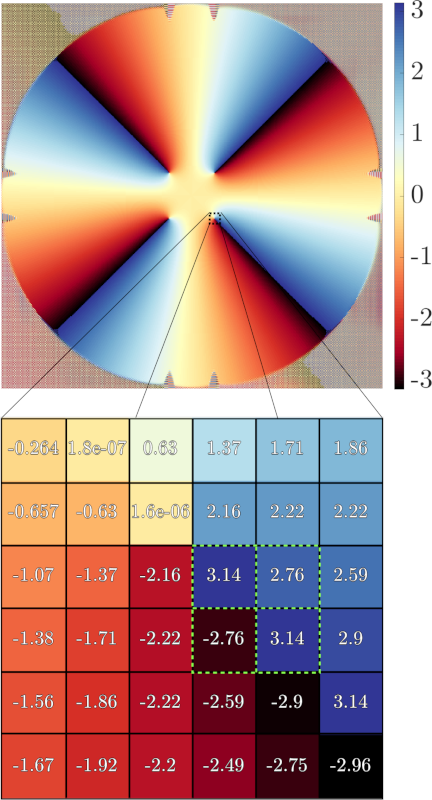
\includegraphics[width = 0.5\textwidth]{data/gpu/vortex_tracking/phi_grid.png}
\caption{An example phase plot of a condensate with four vortices.
The inset shows the values of the phase at each location each vortex location and highlights where the sum is $2\pi$ for vortex tracking.
This image can be found in the GPUE documentation~\cite{docs}.
}
\label{fig:phase_track}
\end{figure}

Instead, the phase can be used to uniquely identify vortex locations, as shown in Figure~\ref{fig:phase_track}.
In the highlighted region, all elements sum to a value of $2\pi$.
In this way, vortex tracking essentially transforms into the task of locating all the $2\pi$ phase windings in the simulated domain via minimization routines where we attempt to find any four grid elements whose sum is $2\pi$.
This process also necessitates a mask for regions outside of the BEC domain, as these regions create spurious $2\pi$ phase windings because of the density is roughly zero outside of the condensate region. 
Further discussion on how to refine this position can be found in previous work~\cite{o2017, docs}.

In three dimensions, vortices are no longer confined to a plane and can extend in any direction, so long as the vortex lines either end at the superfluid surface or reconnect in the form of vortex rings or more complicated vortex structures.
Tracking three-dimensional vortices is a much more difficult problem which does not have many solutions in superfluid simulations where the superfluid does not fill the simulation domain.
The current state-of-the-art solution has been proposed by Villois \textit{et al.}~\cite{villois2016}, and requires finding density dips in the superfluid as initial guesses as to where a vortices might exist.
From there, a vorticity plane is determined and the entire vortex is discovered by moving perpendicularly to the vorticity plane at each gridpoint.
This is a tedious and time-consuming process that does not lend itself well to GPGPU computation without communication between the host and device.
Because some systems simulated with GPUE do not fill the contents of our simulation domain, the proposed method will not work without some modification.
This method could still be used if one has some understanding of the trapping geometry to mask out regions beyond the condensate density; however, as we discussed in Chapter~\ref{ch:splitop}, this is not always the case with gauge fields.
As such, we are currently seeking a more computationally efficient method for tracking vortices in three dimensions, and some thoughts on how this could be done can be found in the Conclusion~\ref{ch:conclusion}.

\begin{figure}
\center 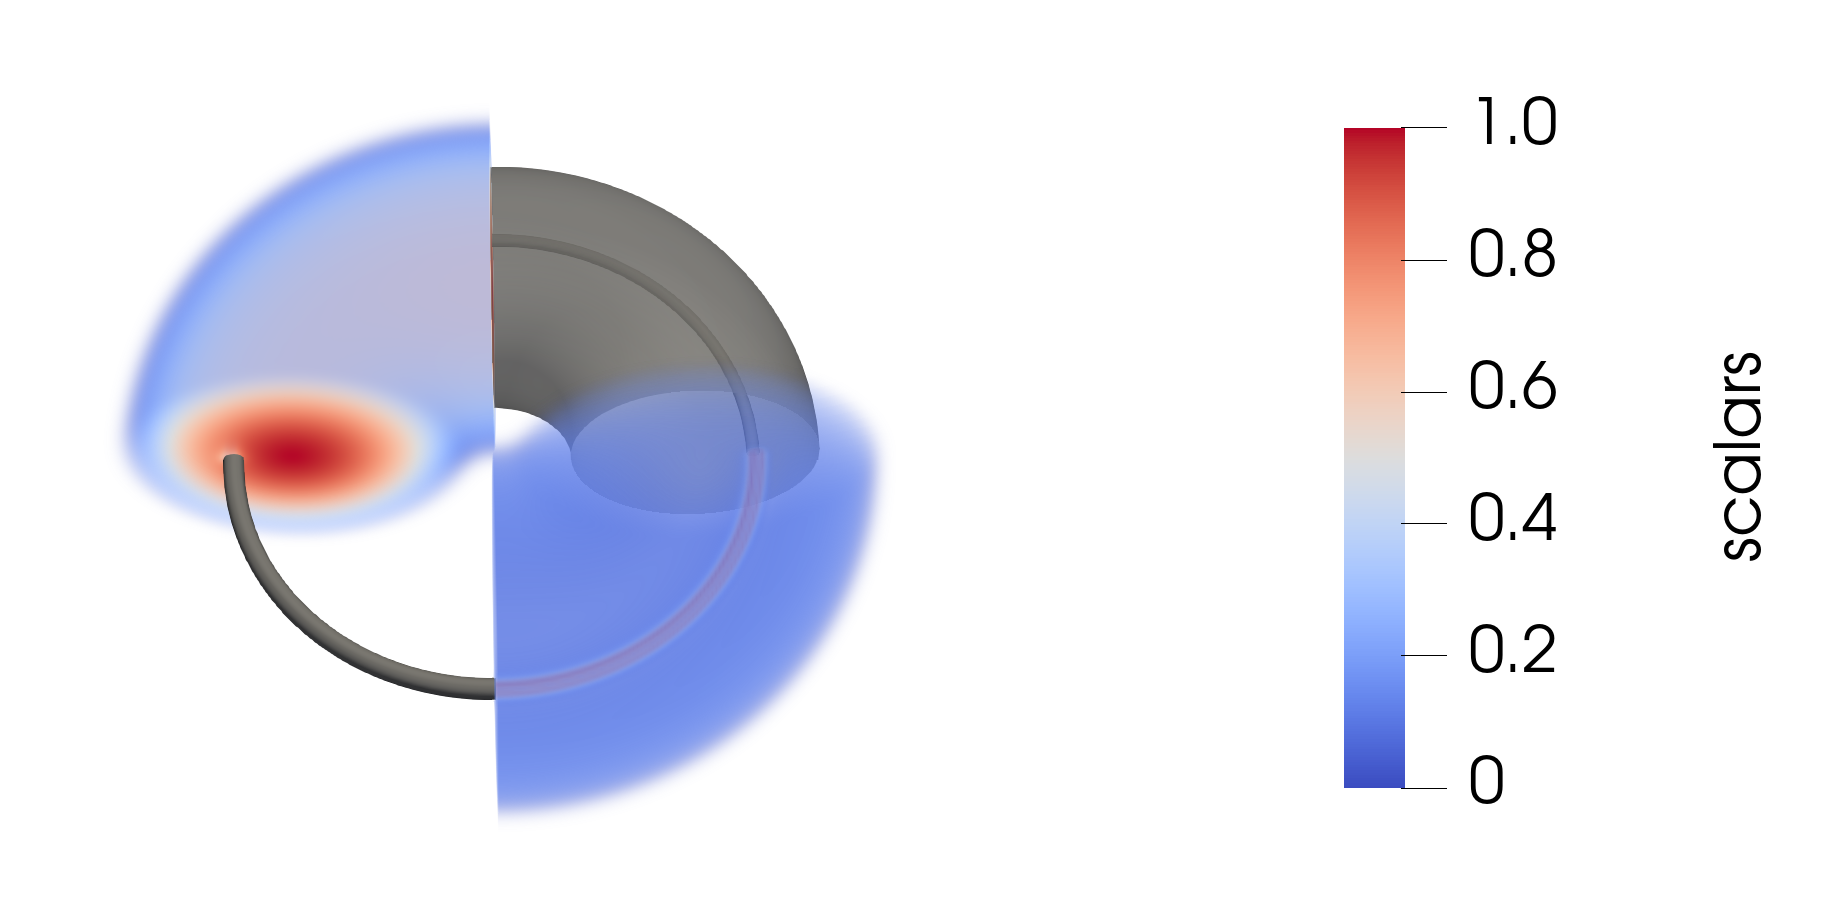
\includegraphics[width=0.75\textwidth]{data/gpu/vortex_highlighting/all.png}
\caption{
An example of vortex highlighting with a Sobel filter.
The upper left quadrant is the superfluid density with no modifications and the upper right quadrant is an isosurface of the density with an opacity of 0.6.
Note here that if there is no opacity set, it is not possible to see the vortex because it is obscured by the outside boundary of the BEC.
The lower right quadrant is the superfluid density after Sobel filtering and the bottom left quadrant is an isosuface on the Sobel filtered density.
Here, we can easily create isosurfaces of vortices that would be occluded when using the density, alone.
The scale varies depending on whether it is coloring the normalized wavefunction density or the filtered density.
}
\label{fig:highlight}
\end{figure}

For these reasons, instead of focusing on vortex \textit{tracking}, I have instead implemented a simple vortex \textit{highlighting} scheme for three dimensions.
This can be done with a Sobel filter on the condensate density, and can easily create crisp visualizations like those found in the computer graphics literature~\cite{guo2018}.
An example of a vortex highlighted wavefunction density, along with an isosurface of both the density and the highlighted density can be seen in Figure~\ref{fig:highlight}.
In this figure, we show that the density after being Sobel filtered can be more easily used to isolate vortex structures without the background BEC.
Though it would be possible to use further edge detection methods, such as the Canny edge detector~\cite{canny1986}, this would add a significant computational overhead and thus was not implemented in the current work.
The problem of efficiently tracking vortex skeletons in three-dimensions is a difficult problem that requires further study; however, vortex highlighting is enough for most three dimensional vortex simulations.
In Chapter~\ref{ch:vortex_states}, we show and example simulation where vortex highlighting has been used to determine the vortex isosurfaces.

\subsection{Energy calculation for superfluid simulations}

As discussed in Chapter~\ref{ch:splitop}, energy calculations can play an essential role in SSFM simulations and can be used to help understand vortex dynamics in certain simulations.
More importantly, energy calculations lie at the heart of convergence criteria for imaginary time propagation.
Essentially, in order to avoid unnecessary computation, many SSFM implementations will cease simulating the system in imaginary time when the change in energy at every timestep drops below a certain threshold value.
Though this option is available in GPUE, it is not a native feature for at least three important reasons:

\begin{enumerate}
\item Certain systems, such as large vortex lattices with high rotation, seemingly have many near-degenerate ground states with different vortex configurations~\cite{o2017, o2016, o2016topo}.
\item GPUE is often run on a computing cluster where the maximum simulation time is set before-hand.
For this, the user must be able to estimate the duration of their simulation, and this is not straightforward if imaginary-time propagation finishes at an unknown time.
\item The energy calculation is memory and operation-intensive and requires at least one additional object of the size of the wavefunction to be created and stored on GPU memory.
\end{enumerate}

\noindent The first and second of these are somewhat self-explanatory, but the third requires further elucidation.

Energy calculations in GPUE are essentially composed of the following operation,

\begin{equation}
E = \braket{\Psi|\mathcal{\hat H}|\Psi}
\end{equation}

\noindent The first problem with this operation is that it requires a summation for the final energy value, and as discussed, this is a poorly-suited problem for GPU hardware.
Even though a robust implementation of parallel reduction has exists in GPUE, this is still a slow process.
The next problem comes from the nature of the Hamiltonian, itself.
As described in Chapter~\ref{ch:splitop}, the Hamiltonian is essentially composed of three separate components for vortex simulations:

\begin{align}
\mathcal{\hat H}_v &= V_0 + g|\Psi|^2 + \frac{m\mathbf{A}^2}{2} \\
\mathcal{\hat H}_p &= \frac{p^2}{2m} \\
\mathcal{\hat H}_{pv} &= p\mathbf{A}
\end{align}

\noindent where $\mathcal{\hat H}_v$, $\mathcal{\hat H}_p$, and $\mathcal{\hat H}_{pv}$ are the Hamiltonians in position-space, momentum-space, and mixed-space, respectively.
These operations can be considered with expression trees; however, for three-dimensional simulations they still require either a set of forward and inverse FFT's or a derivative function with fixed stride along with the parallel reduction operation.
This ultimately amounts to the same number of operations required for a single step of imaginary-time evolution; however, because the simulated wavefunction cannot be influenced by the energy calculation, the operation requires at least one additional allocation of a wavefunction-sized array.
Due to the computational time required for each energy calculation, users are requested to input the set of timesteps they would like to compute the energy for before-hand.
In addition, at certain points, it is impossible to run GPUE with the energy calculation, simply because there is not enough memory available on the device.

Though finding the energy of the wavefunction is a useful feature for certain simulations, it should not be used regularly for memory-limited tasks or tasks that should be performed quickly.
Even so, for most applications of GPUE on HPC environments, there should be no problem running the energy-calculation alongside the simulation, itself.

\subsection{Future direction and multi-GPU development}
\label{sec:multiGPU}

At this point, I would consider GPUE to be close to feature-complete.
It is capable of simulating a wide-variety of quantum systems and can even perform dynamic quantum engineering studies with minimal file input and output.
Though more work can be done to maximize instruction throughput, this will not significantly improve the performance of the code because it relies heavily on double-precision.

The next logical step for GPUE development is scaling to larger simulations.
This means that we either need to increase the number of GPUs used for the simulation or decrease the size of the wavefunction, itself.
Though the CSSFM method~\cite{bayindir2015} should allow for the latter, it was ultimately found unsuitable for general-purpose simulations.
As such, the next logical progression is to scale GPUE to multiple GPU devices; however, as I hope to have impressed by now, this is not a trivial task.
Even though the CuFFT library can support multiple GPU devices, this comes with a huge performance penalty because it lacks an in-built, distributed transpose.
In addition, the \texttt{cufftPlanMany(...)} functionality is unavailble on multiple GPU systems.
To scale to multiple GPU devices efficiently, while still using the SSFM, a large-scale, in-place, multi-GPU transpose is required to ensure proper memory coalescence for FFT routines, which eliminates the need for \texttt{cufftPlanMany(...)} in GPUE.
A transpose of this nature is performed at some step with the CuFFT library; however, unlike FFTW, this step is not outward facing and cannot be controlled by the user.
In addition, the CuFFT library does not allow proper control over the threads designated in each grid when performing largescale allocations of data on multi-GPU memory.

In other languages, like Julia, provide more robust features for distributed GPU computation, and 
for this reason, development of GPUE.jl has begun.
Currently, GPUE.jl has similar performance to GPUE, but is currently lacking the expression tree functionality.
Once GPUE.jl is at feature parity with GPUE, it will become the primary software package for future development.
Ultimately, the Julia language allows for the development of GPUE in a much more maintainable fashion, and also allows for the accessing of GPU hardware in a more convenient way.
In addition to this, Julia allows for more modular development of certain features, such as the DistributedTranspose.jl package that should allow for multi-GPU transposes when fully developed.

\section{DistributedTranspose.jl}
\label{sec:DT}

At its heart, the two-dimensional transpose is a straightforward operation consisting of a swapping of all row and column elements.
Unsurprisingly, this is a difficult task to ensure memory coalescence, but
it is possible to perform a two-dimensional transpose at the same performance as a simple copy, so long as the operation is out-of-place in memory, the operation is performed on shared memory tiles, and bank conflicts are avoided by padding the data structure being transposed~\cite{harris2013}
The transpose becomes even more difficult to create when we wish to transpose large three-dimensional matrices, potentially spanning across multiple GPU devices, while also ensuring the operation is in-place in memory.

In principle, there are three types of three-dimensional transposes:

\begin{description}
\item[Simple Copy]{A benchmark for other transpositions,
    \begin{align}
    A_{xyz} &\rightarrow A_{xyz}
    \end{align}}
\item[Involution]{A transpose where a two-dimensional transpose is operated on a three-dimensional data structure,
    \begin{align}
    A_{x\mathbf{yz}} &\rightarrow A_{x\mathbf{zy}} \\
    A_{\mathbf{xy}z} &\rightarrow A_{\mathbf{xy}z} \\
    A_{\mathbf{x}y\mathbf{z}} &\rightarrow A_{\mathbf{z}y\mathbf{x}}
    \end{align}}
\item[Rotation]{A fully three-dimensional transpose,
    \begin{align}
    A_{\mathbf{xyz}} &\rightarrow A_{\mathbf{yzx}} \\
    A_{\mathbf{xyz}} &\rightarrow A_{\mathbf{zxy}}
    \end{align}}
\end{description}

It has been shown that for out-of-place transpositions, it is possible to perform all of these operations as efficiently as a a simple copy; however, in-place rotational transposes can only attain 60-70\% of the performance based on currently known methods~\cite{jodra2015, el2008}.
In addition, distributed transposes of this nature have not been discussed except for on an out-of-place array~\cite{ruetsch2013}.

At its current state, the DistributedTranspose.jl package is able to do out-of-place, distributed transposes; however, when feature-complete, it should allow for the implementation of new distributed methods for such computation.
It should be mentioned that this package has potential to be used by many other software packages that require using spectral methods on multiple GPU devices.
Often, HPC engineers prefer finite-element or difference methods when computing large-scale fluid flow because these methods scale much better across distributed systems; however, with an appropriate distributed transpose methods, it might be more optimal to perform spectral and pseudo-spectral simulations in certain regimes over other methods.

\section{Outlook}

In this chapter, I presented the fundamentals of GPGPU, along with the GPUE codebase for simulating superfluid vortex systems.
It is important to note that GPU architecture is best at embarrassingly parallel tasks, and as such, the SSFM is severely limited by its FFT routines; however, because one-dimensional FFT operations on GPU devices are often faster for larger matrix sizes than their CPU-based counter-parts~\cite{merz2016}, it seems that the SSFM is better suited for GPU architecture.
In this chapter, I also discussed important optimizations done in GPUE to ensure proper utilization of GPU architecture for dynamic simulations of dynamic superfluid vortex simulations in two and three dimensions, including expression trees, FFT optimizations, vortex tracking and highlighting, methods used to decrease GPUE's storage footprint, and GPUE.jl.
Finally, I discussed the future development of the DistributedTranspose.jl package, which should allow for large-scale spectral methods to be suitable for distributed GPU systems, often found in HPC environments.
Though not mentioned here, GPUE has also been extended for multicomponent simulations, and there is a wide variety of physical systems that can be simulated with this feature, some of which will be mentioned in the Conclusion~\ref{ch:conclusion}.

A really interesting question involved scaling GPUE to become a more general-purposes quantum simulator, similar to XMDS~\cite{dennis2013}.
In comparison to XMDS, GPUE uses the pseudo-spectral SSFM method, while XMDS uses a variety of methods, depending on the task at-hand, primarily relying on interaction-picture methods, such as RK4IP~\cite{murray2011}.
In addition, the XMDS user interface is entirely in XML, which is slightly more cumbersome to the user, but much easier for development.
If GPUE is to scale and become a broader, general-purpose library beyond the GPE and Schr\"odinger equation, more work has to be done to extend the current framework.
As an important note, even though future development for GPUE.jl will be in Julia, the GPUE codebase has been written to minimize the amount of code users will see when simulating superfluid BEC systems.
As such, transitioning to Julia will not radically change the user-interface for GPUE, but will instead serve as a way for developers to write more maintainable code for largescale, multi-GPU simulations in the future.
In addition, GPUE.jl will become a useful tool for users who wish to perform post-processing metrics in the same environment as GPUE, itself, potentially eliminating some file output.
For Chapters~\ref{ch:2d} and \ref{ch:vortex_states}, I will discuss two physical examples that were enabled by the GPUE codebase, also highlighting future physical directions and re-enforcing the future directions discussed here.
